%versi 2 (8-10-2016) 
\chapter{Pendahuluan}
\label{chap:intro}
   
\section{Latar Belakang}
\label{sec:label}

Perangkat lunak KIRI (lihat Gambar \ref{fig:kiri}) adalah perangkat lunak berbasis web yang dirancang untuk membantu pengguna menemukan rute perjalanan menggunakan angkot. Pada perangkat lunak KIRI, pengguna dapat memasukkan titik awal perjalanan dan titik tujuan. KIRI kemudian akan mencarikan berbagai alternatif rute angkot yang bisa digunakan untuk mencapai tujuan tersebut. KIRI akan memberikan informasi mengenai langkah-langkah yang harus ditempuh oleh pengguna yang akan berpergian dari satu tempat ke tempat tujuannya, mulai dari seberapa jauh pengguna harus berjalan untuk menaiki angkot yang bersangkutan, di mana pengguna harus naik atau turun angkot tersebut, seberapa jauh lagi pengguna harus berjalan sampai ke lokasi tujuan, dan seberapa lama estimasi waktu perjalanan yang akan ditempuh.
\begin{figure}[h] 
	\centering  
	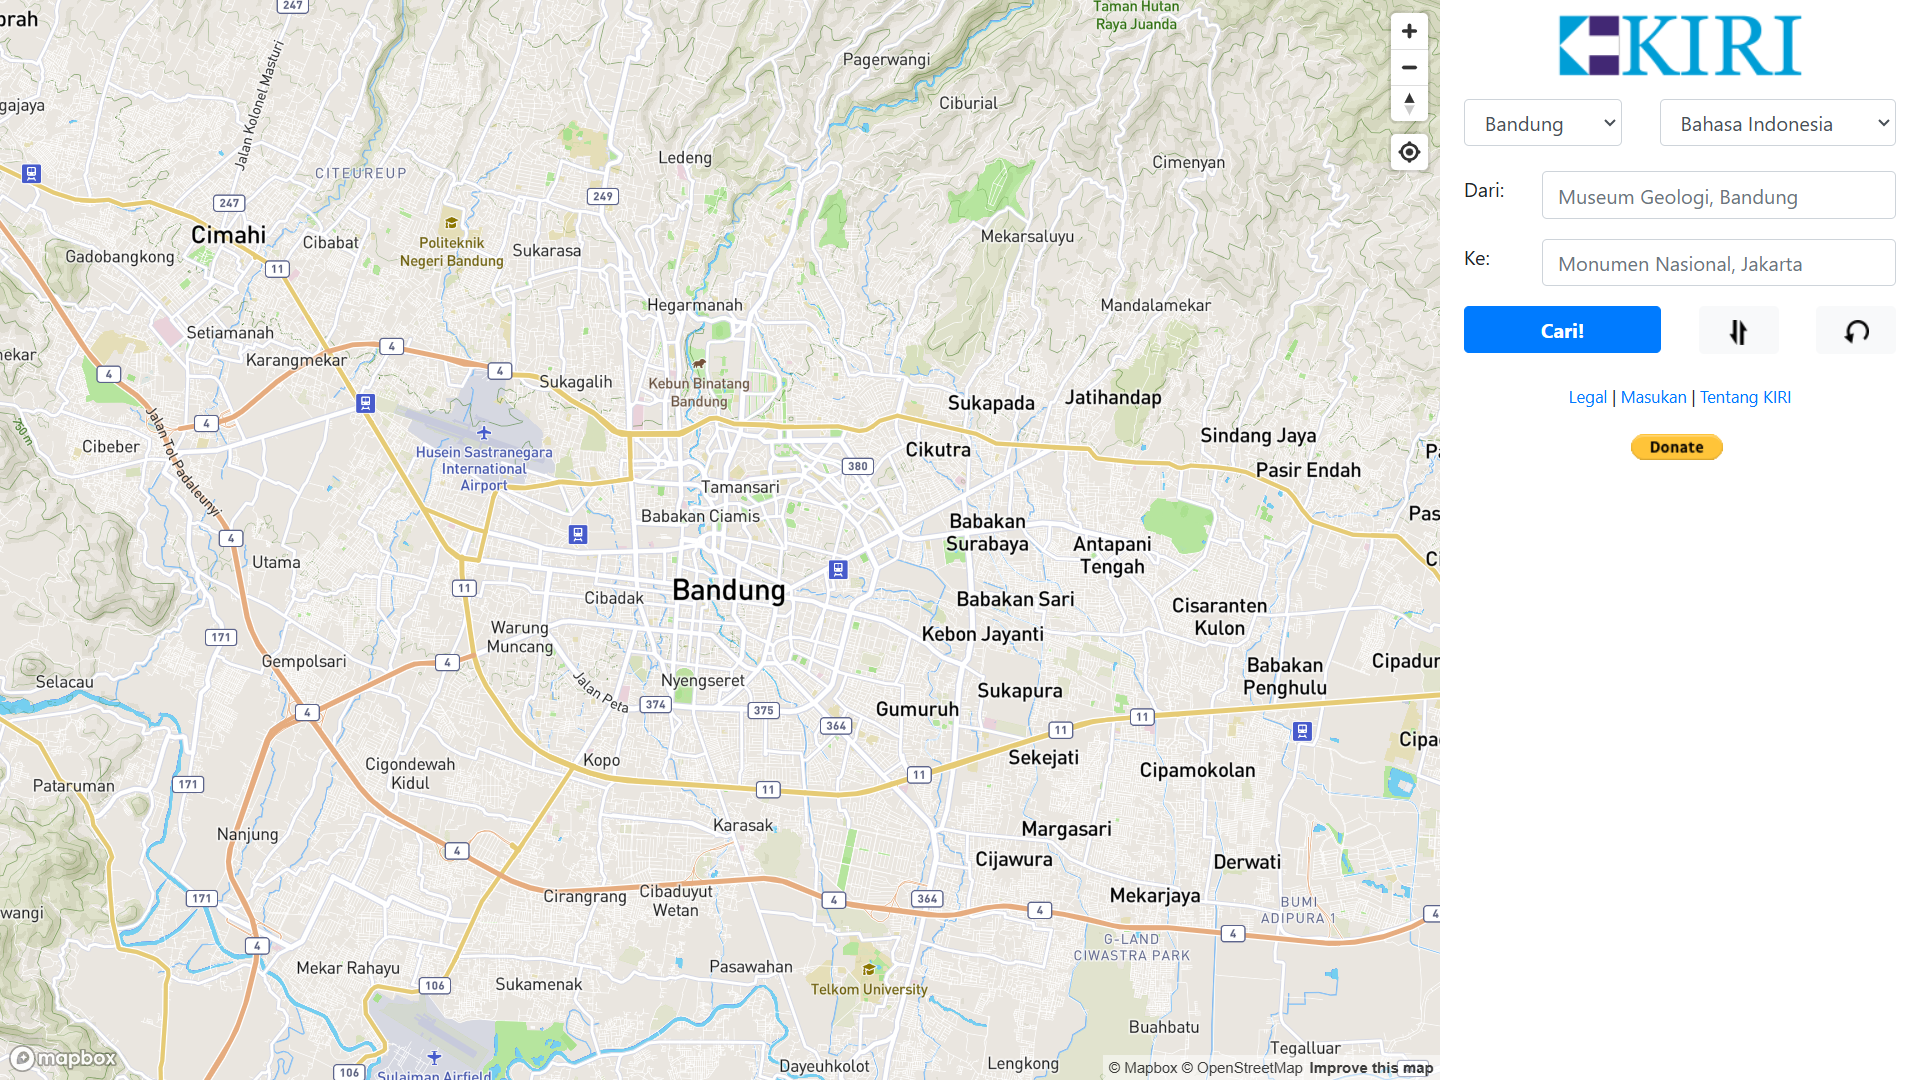
\includegraphics[width=1\textwidth]{KIRI}  
	\caption{Tampilan halaman perangkat lunak KIRI}
	\label{fig:kiri} 
\end{figure}
\newpage
\noindent
Arsitektur aplikasi KIRI terbagi menjadi dua bagian utama. Bagian frontend, yang dinamakan Tirtayasa, dibangun menggunakan bahasa pemrograman PHP dan mengandalkan basis data MySQL untuk menyimpan serta mengelola data. Selain itu, Tirtayasa juga menggunakan framework CodeIgniter 3. Saat menerima permintaan pencarian, Tirtayasa meneruskannya ke bagian backend, yaitu NewMenjangan. Hasil dari NewMenjangan kemudian diformat agar dapat dibaca dengan baik oleh pengguna. Bagian ini diimplementasikan dalam bahasa pemrograman Java dan berperan penting dalam perhitungan rute optimal.
\\
NewMenjangan merupakan program daemon yang berjalan secara otomatis saat server dinyalakan dan terus beroperasi hingga server dimatikan. Daemon sendiri adalah program komputer yang berjalan di latar belakang dan tidak berinteraksi langsung dengan pengguna\footnote{\url{https://www.ibm.com/docs/en/aix/7.1?topic=processes-}}. Pada saat eksekusi, NewMenjangan terhubung ke basis data MySQL untuk mengambil data rute angkot yang tersimpan dalam format \textit{LineString}. \textit{LineString} adalah salah satu tipe data geometris dalam MySQL yang mewakili satu atau lebih segmen garis yang terhubung. \textit{LineString} terdiri dari urutan titik (point) yang membentuk jalur atau lintasan\footnote{\url{https://dev.mysql.com/doc/refman/8.4/en/gis-linestring-property-functions.html}}. Setiap titik pada \textit{LineString} merepresentasikan lokasi potensial untuk penumpang naik atau turun. Dari data tersebut, NewMenjangan membangun \textit{weighted graph} dalam memori (RAM) dalam bentuk \textit{adjacency list} dan melakukan prakomputasi. Setiap titik pada LineString menjadi \textit{node}, dan antara titik ke-i dan titik ke-(i+1) dihubungkan dengan \textit{edge}. Jika ada dua titik dari rute angkot berbeda yang berdekatan (jarak di bawah konstanta tertentu), maka dibuatkan juga \textit{edge}, yang menunjukkan kemungkinan seseorang dapat turun dari suatu angkot dan naik ke angkot lainnya untuk meneruskan perjalanan. 
\\
Saat NewMenjangan menerima permintaan pencarian dari titik A ke titik B, kedua titik tersebut dijadikan \textit{node} sementara, dan dibuatkan \textit{edge} sementara ke \textit{node-node} yang sudah ada sebelumnya, jika jaraknya di bawah konstanta tertentu. Pencarian jarak terdekat pada graf tersebut dilakukan menggunakan algoritma Dijkstra versi teroptimasi (\textit{priority queue} dengan struktur data \textit{heap}). Proses ini dapat dilakukan secara paralel dengan aman (\textit{thread-safe}) tanpa mengubah graf utama.
\\
Pada saat ini algoritma yang digunakan KIRI masih terikat dengan algoritma Dijkstra. Oleh karena itu, pada tugas akhir ini akan diimplementasikan algoritma lainnya, yaitu algoritma A-star dan Floyd Warshall sebagai \textit{concrete strategy}. Selain itu, akan dilakukan juga penerapan arsitektur kelas \textit{strategy pattern} sehingga aplikasi KIRI akan menjadi lebih fleksibel dalam pemilihan algoritma \textit{shortest path} yang akan digunakan dan juga memudahkan apabila akan dilakukan perubahan atau perbaikan pada suatu algoritma yang digunakan.

\section{Rumusan Masalah}
\label{sec:rumusan}
	\begin{enumerate}
                \item Bagaimana cara melakukan perubahan kode pada NewMenjangan untuk menerapkan \textit{strategy pattern}?
                \item Bagaimana mengimplementasikan algoritma A-star dan Floyd Warshall sebagai \textit{concrete strategy}?
	\end{enumerate}
\newpage
\section{Tujuan}
\label{sec:tujuan}
	\begin{enumerate}
                \item Melakukan perubahan arsitektur kelas dengan menerapkan \textit{strategy pattern}.
                \item Melakukan implementasi algoritma A-star dan Floyd Warshall.
            \end{enumerate}

\section{Batasan Masalah}
\label{sec:batasan}
...

\section{Metodologi}
\label{sec:metlit}
Metodologi yang akan digunakan dalam pembuatan tugas akhir ini adalah sebagai berikut:
	\begin{enumerate}
		\item Melakukan eksplorasi fungsi-fungsi dan cara kerja perangkat lunak KIRI.
		\item Mempelajari modul-modul yang terdapat pada Tirtayasa dan NewMenjangan.
		\item Mempelajari bahasa pemrograman PHP dan framework CodeIgniter 3.
		\item Melakukan studi literatur mengenai penerapan arsitektur kelas \textit{strategy pattern}.
    		\item Mempelajari cara kerja algoritma Dijkstra, A-star, dan Floyd Warshall.
    		\item Mengubah implementasi algoritma Dijkstra yang sudah ada ke dalam \textit{strategy pattern}.
    		\item Mengimplementasikan algoritma A-star dan Floyd Warshall.
    		\item Melakukan pengujian dan eksperimen.
    		\item Menulis dokumen tugas akhir.
	\end{enumerate}

\section{Sistematika Pembahasan}
\label{sec:sispem}
Tugas akhir ini akan disusun menjadi beberapa bab sebagai berikut:
	\begin{itemize}
		\item \textbf{Bab 1:} Pendahuluan
		\\ Bab ini berisi latar belakang, rumusan masalah,tujuan, batasan masalah, metodologi, dan sistematika pembahasan.
		\item \textbf{Bab 2:} Landasan Teori
		...
		\item \textbf{Bab 3:} Analisis
		...
	\end{itemize}